%%
%% Author: Alicia Zamorano
%% 21-04-18
%%

% Preamble
\documentclass{article}

% Packages
\usepackage{graphicx}
\usepackage{float}
\usepackage{enumitem}
\graphicspath{{../images/}}

% Document
\begin{document}
\title{Object Oriented Representation of ER Idioms}
\author{Alicia Zamorano}
\maketitle
It is possible to represent complex structures in E-R that represents kinds of
equivalences with OO structures. Developers have found some structures that are
repeated in ER, and this structures can be reused during the development process.
This structures had been used to define a set of \textit{Idioms}\cite{ER_Idioms}.

To be able to understand the existing gap between OO model and ER model is
necessary to depict the \textit{Idioms} using OO model, on this way the
particularities of each representation will be clearly distinguishable resulting
in a set of advantages and disadvantages of each representation.

\section{Setting the Scene}
To establish a point of departure, an example of University data base is shown
in Fig. 1 to lay some groundwork on which the rest of the representation of
\textit{Idioms} can be build.

\begin{figure}
	\centering
	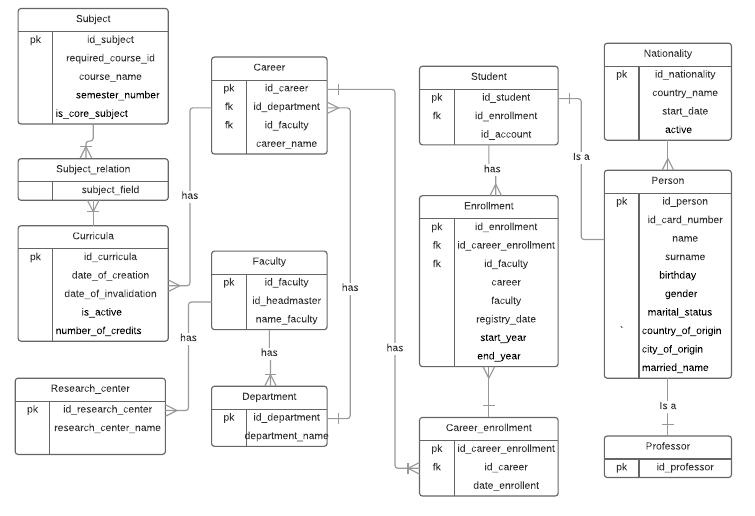
\includegraphics[width=15cm]{universityerdidioms}
	\caption{Entity Relationship Diagram of a University.}
\end{figure}

To elaborate:
\begin{itemize}[label={}]
	\item \textit{Student}\\
	      Student entity denotes the students that are enrolled in the University.
	      Each student has a \{id\_student\} that identifies an student, which is
	      unique and the primary key, an \{id\_register\} which is a foreign key
	      corresponding to the primary key of Student\_register entity.
	\item \textit{Student\_enrollment}\\
	      Student\_enrollment denotes the enrollment registry of a student, each
	      enrollment has an \{id\_enrollment\} that identifies an Student\_enrollment
	      which is the primary key, an \{id\_career\_enrollement\} which is a foreign
	      key corresponds to the primary key of Career\_enrollement, also an
	      \{id\_faculty\} that corresponds to the primary key of Career\_enrollment entity

	\item \textit{Person}\\
	      Person entity denotes each person information that is going to stored in
	      the univerity it has a \{id\_person\} that is the primary key of the entity
	      and identifies each person.
	\item \textit{Professor}\\
	      Professor entity that is at the same time a \textit{person} has an id\_pro
	      fessor that identifies each professor of the university
	\item \textit{Faculty}\\
	      Faculty entity denotes all the faculties that the university has, each
	      faculty has an \{id\_faculty\} which is the primary key.
	\item \textit{Department}\\
	      Department entity denotes the departments that each faculty has, each
	      department has an \{id\_department\} which is the primary key and it has an
	      \{id\_faculty\} which is a foreign key that corresponds to the primary key
	      of Faculty entity
	\item \textit{Research\_center}\\
	      Research\_center entity denotes the Research Center that each faculty has,
	      it has an \{id\_research\_center\} which is the primary key, also it has
	      an \{id\_faculty\} which is a foreign key that corresponds to the primary key
	      of Faculty entity
	\item \textit{Career}
	      Career entity denotes all the careers that belongs to each departments,
	      it has an \{id\_career\} which is the primary key, also it has an \{id\_department\}
	      that correspond to the primary key of Department entity.
\end{itemize}


\section{Representation of ER Idioms}
A representation of each \textit{idiom} defined in \textbf{Idioms en ER}\cite{ER_Idioms}
will be portrait using OO paradigm, to focus on the differences between those
two representations, in addition, a better understanding of limitations and strengths
of each model will be achieved as a result of the comparison.

\begin{enumerate}
	\item \textbf{Classifier}
	      \begin{figure}[H]
	      	\centering
	      	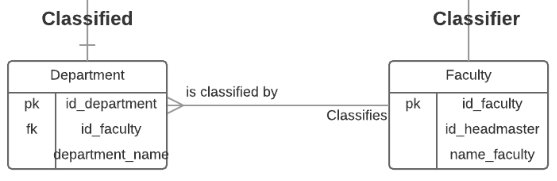
\includegraphics[width=14cm]{classifier}
	      	\caption{Entity Relationship representation of \textit{Idiom} Classifier
	      	using Faculty-Department entities }
	      \end{figure}
	      \begin{figure}[H]
	      	\centering
	      	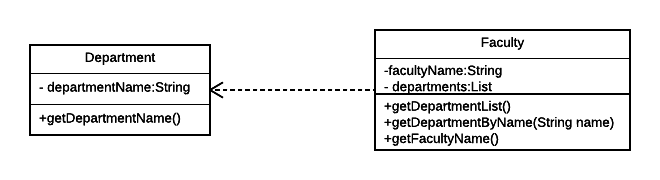
\includegraphics{ooumlclassifier}
	      	\caption{Object Oriented representation of Faculty-Department}
	      \end{figure}
\end{enumerate}

\medskip
\begin{thebibliography}{9}
	\bibitem{ER_Idioms}
	Juan Marcelo Flores Soliz(2006).
	\textit{Idioms en ER. Cochabamba Bolivia:Programa MEMI FCYT, Universidad Mayor de San Simon.}
\end{thebibliography}
\end{document}
